From the given information, 
\begin{align}
\cos B &=\frac{a^2+c^2-b^2}{2ac}
\\
\implies \cos B&=0
\\
\text{or, } \angle B&=90\degree
\end{align}
%
Thus, the vertices of $\triangle ABC$ are 
\begin{align}
\vec{A} = \myvec{0\\2.5}, \vec{B} = \myvec{0\\0}, \vec{C} = \myvec{6\\0}
\end{align}
and plotted in Fig. \ref{triangle/13/fig:triangle ABC}.
%
\begin{figure}[ht]
    \centering
    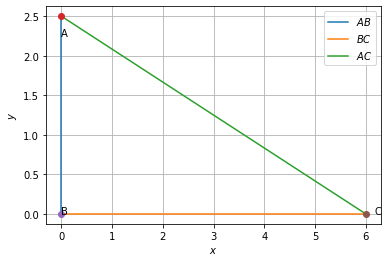
\includegraphics[width=\columnwidth]{solutions/triangle/13/download.png}
    \caption{ $\triangle ABC$}
    \label{triangle/13/fig:triangle ABC}
\end{figure}

